
%%%%%%%%%%%%%%%%%%%%%%%%%%%%%%%%%%%%%%%%%%%%%%%%%%%%%%%%%%%%%%%%%%%%%%%%
%Para las ecuaciones siempre es Ec.(n).
%Para las figuras siempre es Fig.n, incluso en el caption de la figura. Tambien las Tablas
%Para las referencias es [n]
%%%%%%%%%%%%%%%%%%%%%%%%%%%%%%%%%%%%%%%%%%%%%%%%%%%%%%%%%%%%%%%%%%%%%%%%

\documentclass[
reprint,
%notitlepage,
%superscriptaddress,
%groupedaddress,
%unsortedaddress,
%runinaddress,
%frontmatterverbose, 
%preprint,
%showpacs,preprintnumbers,
%nofootinbib,
%nobibnotes,
%bibnotes,
%11 pt,
amsmath,
amssymb,
aps,
pra,
%prb,
%rmp,
%tightenlines %esto hizo el milagro de sacar los espacios en blancos estocásticos (?)
 %prstab,
%prstper,
%floatfix,\textbf{}
]{revtex4-1} %Instalar primero para usarlo. Paquete malo.

%\documentclass[onecolumn, aps, amsmath,amssymb ]{article}
\usepackage{lipsum}  
\usepackage{graphicx}% Include figure files
\usepackage{subfig}
\usepackage{braket}
\usepackage{comment} %comment large chunks of text
\usepackage{dcolumn}% Align table columns on decimal point
\usepackage{bm}% bold math
%\usepackage{hyperref}% add hypertext capabilities
\usepackage[mathlines]{lineno}% Enable numbering of text and display math
%\linenumbers\relax % Commence numbering lines
\usepackage{mathtools} %% Para el supraíndice

\usepackage[nice]{nicefrac}

%%%%%%%El Señor Español%%%%%%%%%%%%%%%%%%%%%%%%%%%
\usepackage[utf8]{inputenc} %acento
\usepackage[
spanish, %El lenguaje.
es-tabla, %La tabla y no cuadro.
activeacute, %El acento.
es-nodecimaldot %Punto y no coma con separador de números
]{babel}
\usepackage{microtype} %para hacerlo más bonito :33 como vos (?) 
%%%%%%%%%%%%%%%%%%%%%%%%%%%%%%%%%%%%%%%%%%%%%%%%%%%
%%%%%%%%% Para que las imágenes se queden dónde las quiero (?
\usepackage{float}
%%%%%%%%%%

%%%%%%%%Cambia a Fig de Figure%%%%%%%%%%
\makeatletter
\renewcommand{\fnum@figure}{Fig. \thefigure} 
\makeatother
%%%%%%%%%%%%%%%%%%%%%%%%%%%%%%%%%%%%%%%%
\raggedbottom


\begin{document}
%%%%%%%%%%%%%%%%%%%%%%%%%%%%%%%%%%Título%%%%%%%%%%%%%%%%%%%%%%%%%%%%%%%%%%%%%%
%%%%%%%%%%%%%%%%%%%%%%%%%%%%%%%%%%%%%%%%%%%%%%%%%%%%%%%%%%%%%%%%%%%%%%%%%%%%%%

\title{Práctica 1}
\author{Evelyn~G.~Coronel}

\affiliation{
Redes Neuronales - Instituto Balseiro\\}

\date[]{\lowercase{\today}} %%lw para lw, [] sin date

\begin{abstract}
Soluciones a los ejercicios de la práctica 1 de la materia de Redes neuronales
\end{abstract} 
\maketitle
%%%%%%%%%%%%%%%%%%%%%%%%%%%%%%%%%%%%%%%%%%%%%%%%%%%%%%%%%%%%%%%%%%%%%%%%%%%%%%%%%%%
% Podemos usar cualquiera de los dos comandos: \input o \include para incluir el texto
%\input{./Capitulo1/cap1.tex}


\section{Ejercicio 1 }

Considerando la ecuación de Nerst dada por la Ec.\,\ref{nerst} y que $\nicefrac{KT}{e}\approx 26 $\,mV , con los datos de la Tabla\,\ref{table_ej1}

	\begin{equation}
		V = \frac{KT}{e} \ln\bigg(\frac{[A]_{out}}{[A]_{in}}\bigg)
		\label{nerst}
	\end{equation}

	\begin{table}[H]
	\centering
	\begin{tabular}{c|c|c|c}
	Elemento & Interior [mM] & Exterior [mM]& V [mV] \\ \hline
	K$^+$	 & 430			 & 20 			& -184.1 \\
	Na$^+$	 & 50 			 & 440			& 130.5 \\
	Cl$^-$	 & 65			 & 550			& 128.1 \\
	\end{tabular}
	\caption{Resultados} \label{table_ej1}
	\end{table}

\section{Ejercicio 2}

La ecuación de Goldmann es la Ec.\,\ref{goldmann}

\begin{equation}
		j_A = \rho_A \frac{q_AV}{KT} \bigg(\frac{[A]_o - [A]_i e^{q_A V / KT}}{1 - e^{q_A V / KT} }\bigg)
		\label{goldmann}
\end{equation}

Renombremos la variable $\frac{eV}{KT}$  como $\frac{eV}{KT} = \alpha$, y la ecuación queda como
\begin{equation}
		j_A = \rho_A \, n_A \alpha \bigg(\frac{[A]_o - [A]_i e^{n_A\alpha}}{1 - e^{n_A\alpha} }\bigg)
\end{equation}

Para los valores de la tabla\,\ref{table_ej1}, considerando las valencias $n_A$ de los elementos, se obtiene las curvas de la Fig.\ref{fig:curvas_ej2}. Es esta figura se observa que si la energía térmica es 5 veces mayor o menor que la energía $qv$, la curva puede aproximarse a una recta.

\begin{figure}[H]
	\centering
	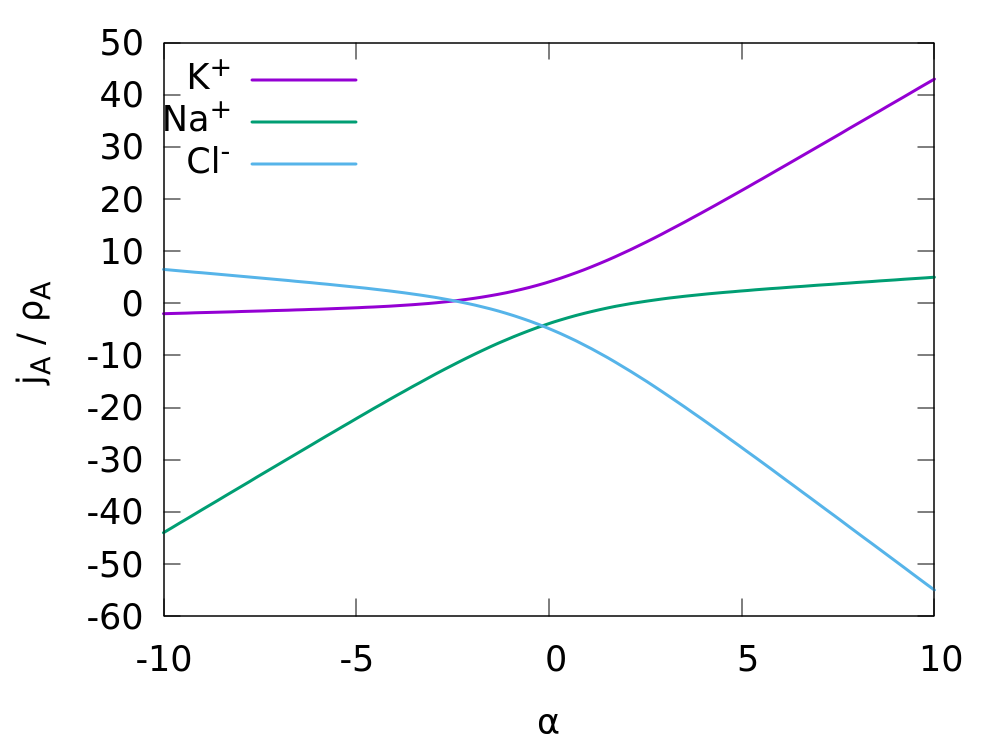
\includegraphics[width=0.5\textwidth]{curvas_ej2.png}
	\caption{Curvas del valor de $\nicefrac{j_A}{\rho_A}$ en función del parámetro $\alpha$}
	\label{fig:curvas_ej2}
\end{figure}

\section{Ejercicio 3}

Considerando que $Q=CV$, entonces

\begin{align*}
    Q=&CV\\
    \Delta Q=& (1 \nicefrac{\mu F}{mm^2} * 4\pi * (15 \mu m)^2) \times \Delta V\\
    \Delta Q=& (1 \nicefrac{\mu F}{mm^2} * 4\pi * (15 \mu m)^2) \times (100 mV)\\   
    \Delta Q=& (1 \times \nicefrac{10^{-6} F}{10^6 \mu m^2} * 4\pi * (15 \mu m)^2) \times (100 mV)\\
    \Delta Q=& (10^{-13} * 4\pi * 15^2)C)\\
    \Delta Q=& 0.283 \times 10^{-9}C\\  
\end{align*}
Esa es la carga: la cantidad de moles de Na son: $0.283 \times 10^{-14}$mol.

\section{Ejercicio 4}

\end{document}